\documentclass[a4paper,10pt]{article}

%linguagem
\usepackage[brazil]{babel}
%encodificação
\usepackage[utf8]{inputenc}
%biblioteca de matemática
\usepackage{amssymb,amsmath}
%pacote para codigo fonte
\usepackage{listings}
%figuras
\usepackage{graphicx}
%cores
\usepackage{color}
%paragrafo no inicio da secao
\usepackage{indentfirst}
%url
\usepackage{framed, url}
\usepackage{fancyvrb}

\usepackage{longtable}

\usepackage[table]{xcolor}
\newcommand{\p}{\cellcolor{blue}}
\usepackage{slashbox} % Linha diagonal na tabela

%define a cor "claro"
\definecolor{claro}{gray}{0.96}

%configurações do fancy verbatim
\fvset{frame=single, xleftmargin=-80pt, xrightmargin=-80pt}
%configurações do listings
\lstset{language=C,frame=trBL, numbers=left, xleftmargin=0pt, xrightmargin=0pt,breaklines=true, backgroundcolor=\color{claro}}

\begin{document}

\begin{titlepage}
\begin{center}


\includegraphics[scale=0.2]{imagens/UFMG.png}\\
\textsc{\LARGE Universidade Federal de Minas Gerais\\
	Departamento de Ciência da Computação}\\[1.5cm]

\textsc{\Large Redes de Computadores\\
	Trabalho Prático 3}\\[0.5cm]

\hrulefill \\[0.4cm]
{ \LARGE \bfseries sistema de mensagens}\\[0.4cm]

\hrulefill \\[1.5cm]
\vspace{7cm}
\begin{minipage}{0.4\textwidth}
\begin{flushleft} \large
\emph{Aluno:}\\
Pedro Araujo Pires \\
\end{flushleft}
\end{minipage}
\begin{minipage}{0.4\textwidth}
\begin{flushright} \large
\emph{Professor:}\\
Luis Felipe Menezes Vieira\\
\end{flushright}
\end{minipage}

\vfill

{\large \today}

\end{center}
\end{titlepage}


\tableofcontents
\pagebreak

\section{Introdução}

Já fazem muitos anos que não conseguimos pensar em um computador como uma
máquina isolada do mundo. As redes permitem a comunicação entre computadores, e
por consequência entre usuários. A Internet não nos deixa dúvidas.

\subsection{Modelo cliente-servidor}
Grande parte da comunicação entre processos é feita utilizando o modelo
cliente-servidor. Este modelo se baseia na ideia de que um processo (o cliente)
se conecta a outro (o servidor) para pedir ou enviar informações. Uma boa
analogia seria uma pessoa fazendo uma ligação telefônica para outra. A pessoa
que faz a ligação precisa de saber o número do telefone da outra, mas quem
recebe não sabe quem está ligando. Uma vez que a chamada é completada, ambas as
pessoas podem falar e/ou escutar. A figura \ref{fig:clienteservidor} ilustra
este modelo.

\begin{figure}[ht!]
\begin{center}
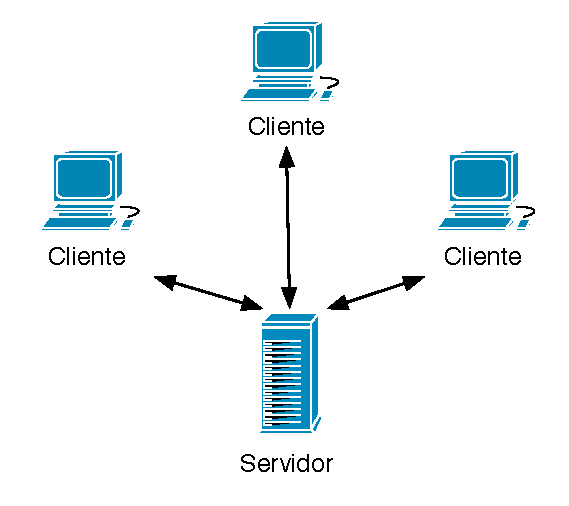
\includegraphics[scale=0.7]{imagens/clienteservidor.pdf}
\label{fig:clienteservidor}
\caption{Modelo cliente-servidor}
\end{center}
\end{figure}

\subsection{Protocolo UDP}
Para trocar informações entre computadores, além de estarem conectados, eles
precisam entender o que representam os dados enviados através da rede. Este é o
papel dos protocolos de rede. A Internet foi projetada através de camadas de
protocolos. Deste modo os desenvolvedores teriam liberdade para criar e mudar as
formas de comunicação sem precisar remodelar toda a estrutura da Internet. O
protocolo UDP - User Datagram Protocol - fica na camada de transporte, como visto na figura
\ref{fig:protocolos}. Isto significa que ele é responsável por passar uma
mensagem vinda da rede para uma aplicação um nível acima. O UDP utiliza a forma
de datagramas para enviar mensagens e não garante a confiabilidade do canal.
Desta forma a aplicação fica responsável pelo tratamento de possíveis erros na
transmissão de pacotes entre o cliente e o servidor.

\begin{figure}[ht!]
\begin{center}
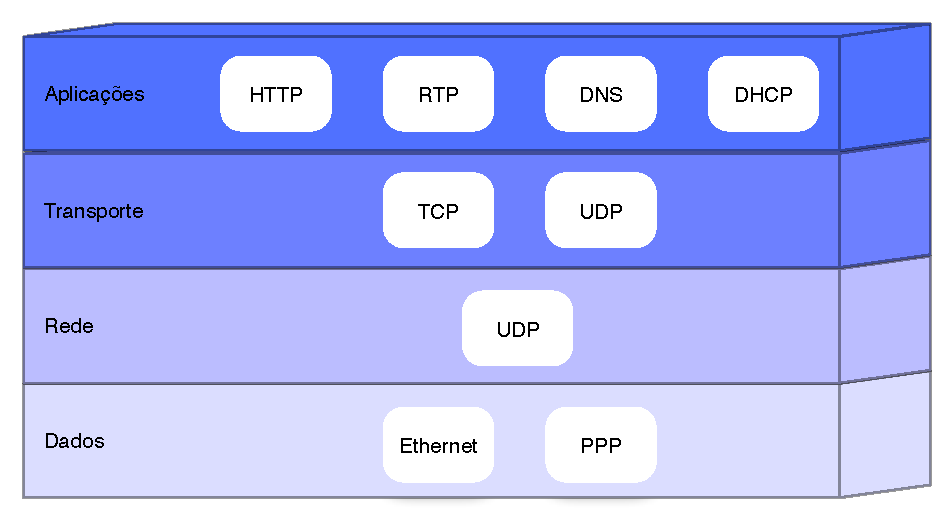
\includegraphics[scale=0.7]{imagens/protocolos.pdf}
\label{fig:protocolos}
\caption{Camadas de protocolos}
\end{center}
\end{figure}

\subsection{Janela Deslizante}

Existem várias formas de estabelecer a confiabilidade da rede, que não é fornecida pelo protocolo UDP. Uma delas é o
método {\it Stop-and-wait}. Basicamente, o transmissor envia cada pacote e espera sua confirmação para então poder
enviar o próximo. A desvantagem deste método é que o canal permanece ocioso enquanto ele funciona com base na premissa
de que antes de enviar um novo pacote, o transmissor deve ter certeza que o receptor recebeu o pacote anterior. Uma
forma de permitir que o canal não fique ocioso é através da utilização de janelas deslizantes. Para isso cria-se {\it
buffers} para armazenar temporariamente os pacotes enviados e recebidos. Assim pode-se enviar pacotes simultaneamente.

\begin{figure}[ht!]
\begin{center}
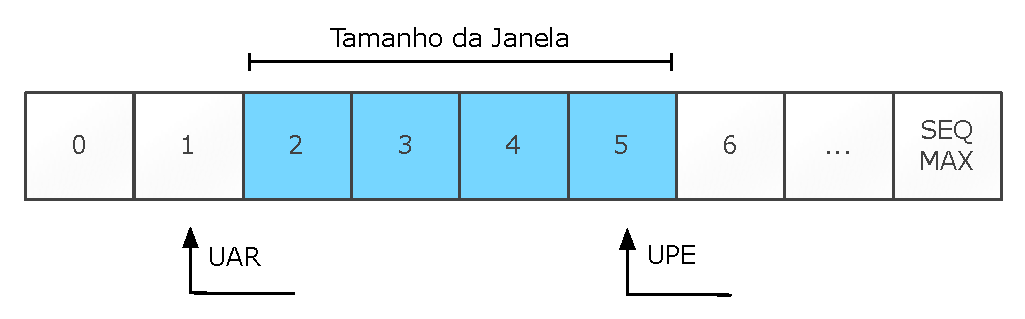
\includegraphics[scale=0.6]{imagens/janela.pdf}
\label{fig:janela}
\caption{Exemplo de protocolo de janela deslizante}
\end{center}
\end{figure}

O objetivo deste trabalho foi desenvolver uma aplicação no modelo cliente-servidor, em cima do protocolo UDP, utilizando
o protocolo de janela deslizante {\it Go-Back-N} (janela do receptor tem tamanho de um pacote). O cliente envia ao
servidor o nome do arquivo que deseja, e recebe este arquivo. Para isto deveria ser usada a biblioteca {\it sockets} do
Unix.

\section{Implementação}

Para a temporização foi utilizado o próprio tempo de {\it timeout} (SO\_RCVTIMEO) da biblioteca {\it sockets} de forma
que, caso não chegue a confirmação do pacote, o mesmo é retransmitido.

São três tipos de mensagens previstas para o protocolo implementado: mensagens de \textit{DADOS}, \textit{ACK}
(confirmações) e {\it FINAL} (para indicar o fim do arquivo). Entretanto, adotou-se um formato único de mensagem a ser
usado nesse protocolo, cuja composição do cabeçalho é dada a seguir:

\begin{itemize}
 \item \textbf{Byte 1-4:} Número do pacote
 \item \textbf{Byte 5:} Tipo de informação do pacote ({\it DADOS}, {\it ACK} ou {\it FINAL}) 
 \item \textbf{Byte 6:} CheckSum (verificação da integridade)
 \item \textbf{Byte 7 em diante:} Flags
\end{itemize}


\begin{figure}[ht!]
\begin{center}
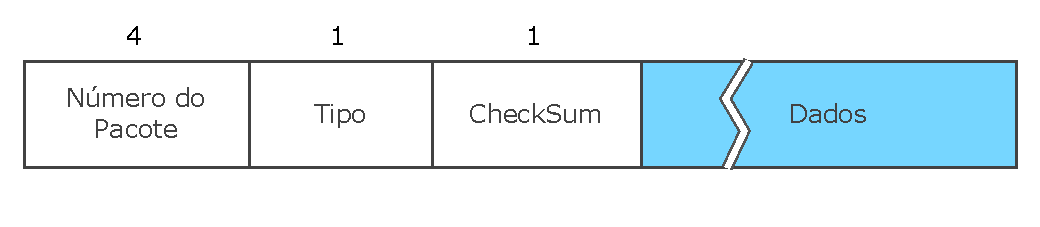
\includegraphics[scale=0.6]{imagens/pacote.pdf}
\label{fig:pacote}
\caption{Pacote do protocolo}
\end{center}
\end{figure}

\subsection{Recuperação de Erros}

O mecanismo de recuperação de erros é baseado no arcabouço fornecido pela temporização. 

\subsubsection{Erro de transmissão}
Ao determinar um tempo de {\it time out} para os pacotes, caso não chegue a confirmação de um pacote esperado ele é
enviado novamente. Isso a princípio pode ser um problema caso um {\it ACK} seja perdido, porém seu pacote relativo tenha
sido recebido com sucesso. Para tratar esse tipo de problema, são definidos contadores que marcam qual é o pacote
esperado. Caso o pacote recebido não seja o esperado temos algumas opções:
\begin{itemize}
  \item {\bf O cliente recebeu um pacote que já foi recebido}: quer dizer que o servidor não recebeu o {\it ACK} daquele
  pacote, logo, descarta-se aquele pacote, porém reenvia o {\it ACK} referente a ele.
  \item {\bf O servidor não recebe nenhum {\it ACK}}: ele deve reenviar todos os pacotes do {\it buffer} antes de mover
  com a janela deslizante pois não se sabe qual pacote não foi recebido pelo cliente.
  \item {\bf O servidor recebe o {\it ACK} de um pacote não esperado}: como foi implementado com {\it Go-Back-N} é certo
  que os pacotes anteriores à esse foram recebidos pelo cliente, então o servido age de acordo.
\end{itemize}

\subsubsection{Checksum} Um \textit{checksum} é anexado ao cabeçalho do pacote antes do envio. No \textit{reciever},
quando um pacote chega, é feito um \textit{checksum} também e os resultados obtido são comparados. Caso os dois não
casarem, o pacote é descartado e com isso o \textit{sender}, ao esperar pela confirmação, tem seu \textit{timeout}
esgotado e retransmite o pacote. O \textit{sender} sempre retransmite um pacote caso a confirmação não chegue antes do
\textit{timeout}, ou seja, o pacote é reenviado.  A recuperação dos dados é feita através dessa retransmissão.


\section{Metodologia}

\subsection{Ambiente de testes}

Os testes feitos foram realizados numa máquina com as seguintes configurações:

\begin{itemize}
\item Processador: Intel(R) Core(TM)2 Duo CPU P8600 @ 2.40GHz
\item Cache: 3072 KB
\item Memória: 3092344 KB
\item Kernel: 2.6.28-19-generic
\end{itemize}

\subsection{Testes}

\subsubsection{Sem erros}
\begin{itemize}
\item Tamanho do arquivo: 2KB
\item Tamanho do buffer: 20B
\item Tamanho da janela: 5
\end{itemize}

\begin{verbatim}
Servidor
*****************************************************************
Total de pacotes enviados: 104
Total de pacotes recebidos: 1
Total de confirmações recebidas: 104
Total de reenvios: 0

Cliente
*****************************************************************
Tempo de execução: 0.006s
Taxa de envio (bytes/s): 3381119.842
Taxa de pacotes (pacotes/s): 17333.333

Total de pacotes enviados: 1
Total de pacotes recebidos: 104
\end{verbatim}

\newpage
\begin{itemize}
\item Tamanho do arquivo: 2KB
\item Tamanho do buffer: 10B
\item Tamanho da janela: 5
\end{itemize}

\begin{verbatim}
Servidor
*****************************************************************
Total de pacotes enviados: 206
Total de pacotes recebidos: 1
Total de confirmações recebidas: 206
Total de reenvios: 0

Cliente
*****************************************************************
Tempo de execução: 0.015s
Taxa de envio (bytes/s): 134763.097
Taxa de pacotes (pacotes/s): 13733.333

Total de pacotes enviados: 1
Total de pacotes recebidos: 206
\end{verbatim}

\subsubsection{Com erros}

\begin{itemize}
\item Tamanho do arquivo: 2KB
\item Tamanho do buffer: 10B
\item Tamanho da janela: 5
\item Taxa de erro: 20\%
\end{itemize}

\begin{verbatim}
Servidor
*****************************************************************
Total de pacotes enviados: 207
Total de pacotes recebidos: 1
Total de confirmações recebidas: 177
Total de reenvios: 1

Cliente
*****************************************************************
Tempo de execução: 1.011s
Taxa de envio (bytes/s): 2025.705
Taxa de pacotes (pacotes/s): 203.7586

Total de pacotes enviados: 1
Total de pacotes recebidos: 206
\end{verbatim}

\newpage
\begin{itemize}
\item Tamanho do arquivo: 2KB
\item Tamanho do buffer: 10B
\item Tamanho da janela: 5
\item Taxa de erro: 50\%
\end{itemize}

\begin{verbatim}
Servidor
*****************************************************************
Total de pacotes enviados: 212
Total de pacotes recebidos: 1
Total de confirmações recebidas: 122
Total de reenvios: 6

Cliente
*****************************************************************
Tempo de execução: 3.014s
Taxa de envio (bytes/s): 679.5415
Taxa de pacotes (pacotes/s): 70.3384

Total de pacotes enviados: 1
Total de pacotes recebidos: 206
\end{verbatim}

\subsection{Resultados}
O que podemos destacar das transmissões com inserção de erros e sem inserção de erros é o grande impacto sobre o
desempenho final da transmissão. Nos testes com a inserção de erro, a duração dos \textit{timeouts} e sua
ocorrência mais frequente principalmente nos arquivos maiores influencia muito no resultado.

Os resultados obtidos atenderam nossas espectativas nos casos testados. Com a inserção de erros a transmissão é mais
demorada devido ao reenvio de pacotes. O \textit{overhead} de espera pelo pacote pode ser bem observado quando variamos
o \textit{timeout} dos pacote.

\section{Conclusões}
O protocolo de janela deslizante apresenta um maior desempenho na rede, pois consegue enviar mais pacotes em um
intervalo de tempo menor. O protocolo pára-e-espera não consegue o mesmo pelo fato de esperar por cada confirmação do
pacote que acabou de enviar, só enviando o próximo quando receber a confirmação do atual, o que resulta em baixa taxa de
utilização da rede e consequente ineficiência na transmissão. Porém, como a função de recebimento causa uma espera no 
programa, esse resultado não é visto no tempo de execução.

O trabalho foi de grande importância para conhecer a complexidade na implementação de protocolos de envio de arquivos. A
teoria envolvida neste trabalho é bem simples, entretanto a implementação possui vários detalhes de funcionamento que a
torna complexa de se codificar.

\clearpage
\begin{thebibliography}{99}
\bibitem{howto} \url{http://www.linuxhowtos.org/C_C++/socket.htm}
\bibitem{slide} \url{http://www.slideshare.net/jignesh/socket-programming-tutorial}
\end{thebibliography}

\end{document}
